\section{Approach} \label{approach}

In this section, we will outline our approach to a linear logic evaluator, describe how we used to it to generate stories in the domain of murder mysteries, while making sure that actors made choices that appear coherent, and finally describe the user interface we built to allow players to interact with the system.

\todo{give an overview of what the game does with a screenshot}

\subsection{Linear Logic Evaluator}\label{own_linear_logic_evaluator}

Our approach on story generation is based on the approach used by the Ceptre story generation engine.
This engine comes with a linear logic evaluator that takes rules that describe the transformation of resources to model the development of a story.
The Ceptre engine is written in the Standard Meta Language and complied via MLton\footnote{http://mlton.org/}.
Early in the project, we used too many constraints, modeled as resources, for Ceptre to handle.
Execution speed would quickly deteriorate, especially as the simulation dragged on.
As a consequence, we decided to implement a version of Ceptre, reduced to the aspects that we were making use of.
This meant that we dropped features like Ceptre's stages and its advanced type system with support for inheritance.
The type system, which allowed for elegant rules like \enquote{has Character gun} for the predicate \enquote{has character object} and the subtype \enquote{gun} of \enquote{object}, made the evaluation considerably more complex as each type instance would increase the possible permutations of each rule making use of it.
For our simple use cases, we were able to avoid using types other than our actors by using rules of the form \enquote{has\_gun Character}.

Our linear logic evaluator takes a set of actors, a set of rules and a set of predicate instances that form the initial state of the simulation.
Predicates have a name and an ordered list of placeholders that can be taken up by any actors.
A predicate instance is a predicate of which all placeholders have been configured with concrete actors.
Rules consist of a left-hand side and a right-hand side, both containing predicates.
The predicate's placeholders are numbered consistently, so that advanced rules that refer to the same actors across the predicates of a rule are possible.
To this extent, our evaluator forms a strict subset of that of Ceptre. 
\todo{more examples}

We extended this system by introducing non-determinism. This means that the right-hand side may list multiple sets of predicates that are all possible outcomes of activating this rule, together with a probability of each outcome occurring. Prior to this, we had two rules for each possible outcome, for example one for stealing from another actor successfully and another for getting caught in the act. This worked fine while randomly selecting rules, but as soon as we started using artificial intelligence to select rules, the agents quickly learned that picking the rule where they get caught was not a good choice.

To further guide the learning intelligence in its decisions, we added a system of rewards to each rule. For each outcome of a rule, the agent could receive a reward or a penalty in different categories.
As categories, we chose \emph{social}, \emph{sanity} and \emph{fulfillment}, loosely based on the top three layers of Maslow's hierarchy of needs \emph{belongingness and love}, \emph{self-esteem and respect} and \emph{self-actualization} \cite{maslow_1943}.
These rewards proved to be general enough so that each rule we developed could have an intuitive value associated with it.
Lastly, we added a built-in templating system that used knowledge embedded in the system to formulate the rules as natural sentences.
This allowed the formulation of templates like this:,
\begin{lstlisting}
Shocked by the revelation that
[0:his|her] [2:husband|wife] was
cheating, {0} murdered [2:his|her]
lover {1}.
\end{lstlisting}
where the each \lstinline|{i}| will be replaced with the name of the i-th actor in the rule and each \lstinline{[i:a|b]} will be replaced by a or b depending on if i-th actor is male or female.

\subsection{A Murder Mystery Rule Set}

As a basis for the rules, we chose to introduce resources that model the current relationships between characters and general tendencies in their character to act in certain ways. For these, we adapted the \emph{Big Five Personality Traits} \cite{rothmann_coetzer_2003}, giving each character a balance of three resources for each opposing pair of traits. For example, a character might receive two \emph{cautious} resources and one \emph{curious} resource, or three \emph{confident} resources and no \emph{insecure} resources. This allowed authoring rules that require a certain tendency towards one of the extremes of each trait pair. To model the relationships between characters, we used \emph{Plutchik's Wheel of Emotion} \cite{plutchik_2001}. Again, we have opposing pairs that are however not necessarily exclusive in our system. Spending time with another actor may yield \emph{trusting} resources between the two, while fighting might yield \emph{anger} resources. A \emph{making up} rule would then allow removing \emph{anger} resources again. To model more extreme characters, we introduced a system similar to alignments as found in some role-playing games. Actors may either be good, neutral or, evil, which will enable them to pick certain options more easily than other characters.

In the next step, we generate relationships and attributes relevant to our domain of murder mystery. This includes whether a character is rich (\enquote{has\_money Character}), their current relationship to other characters using the wheel of emotion, or whether the characters are either related, or lovers or married.

\begin{figure*}
  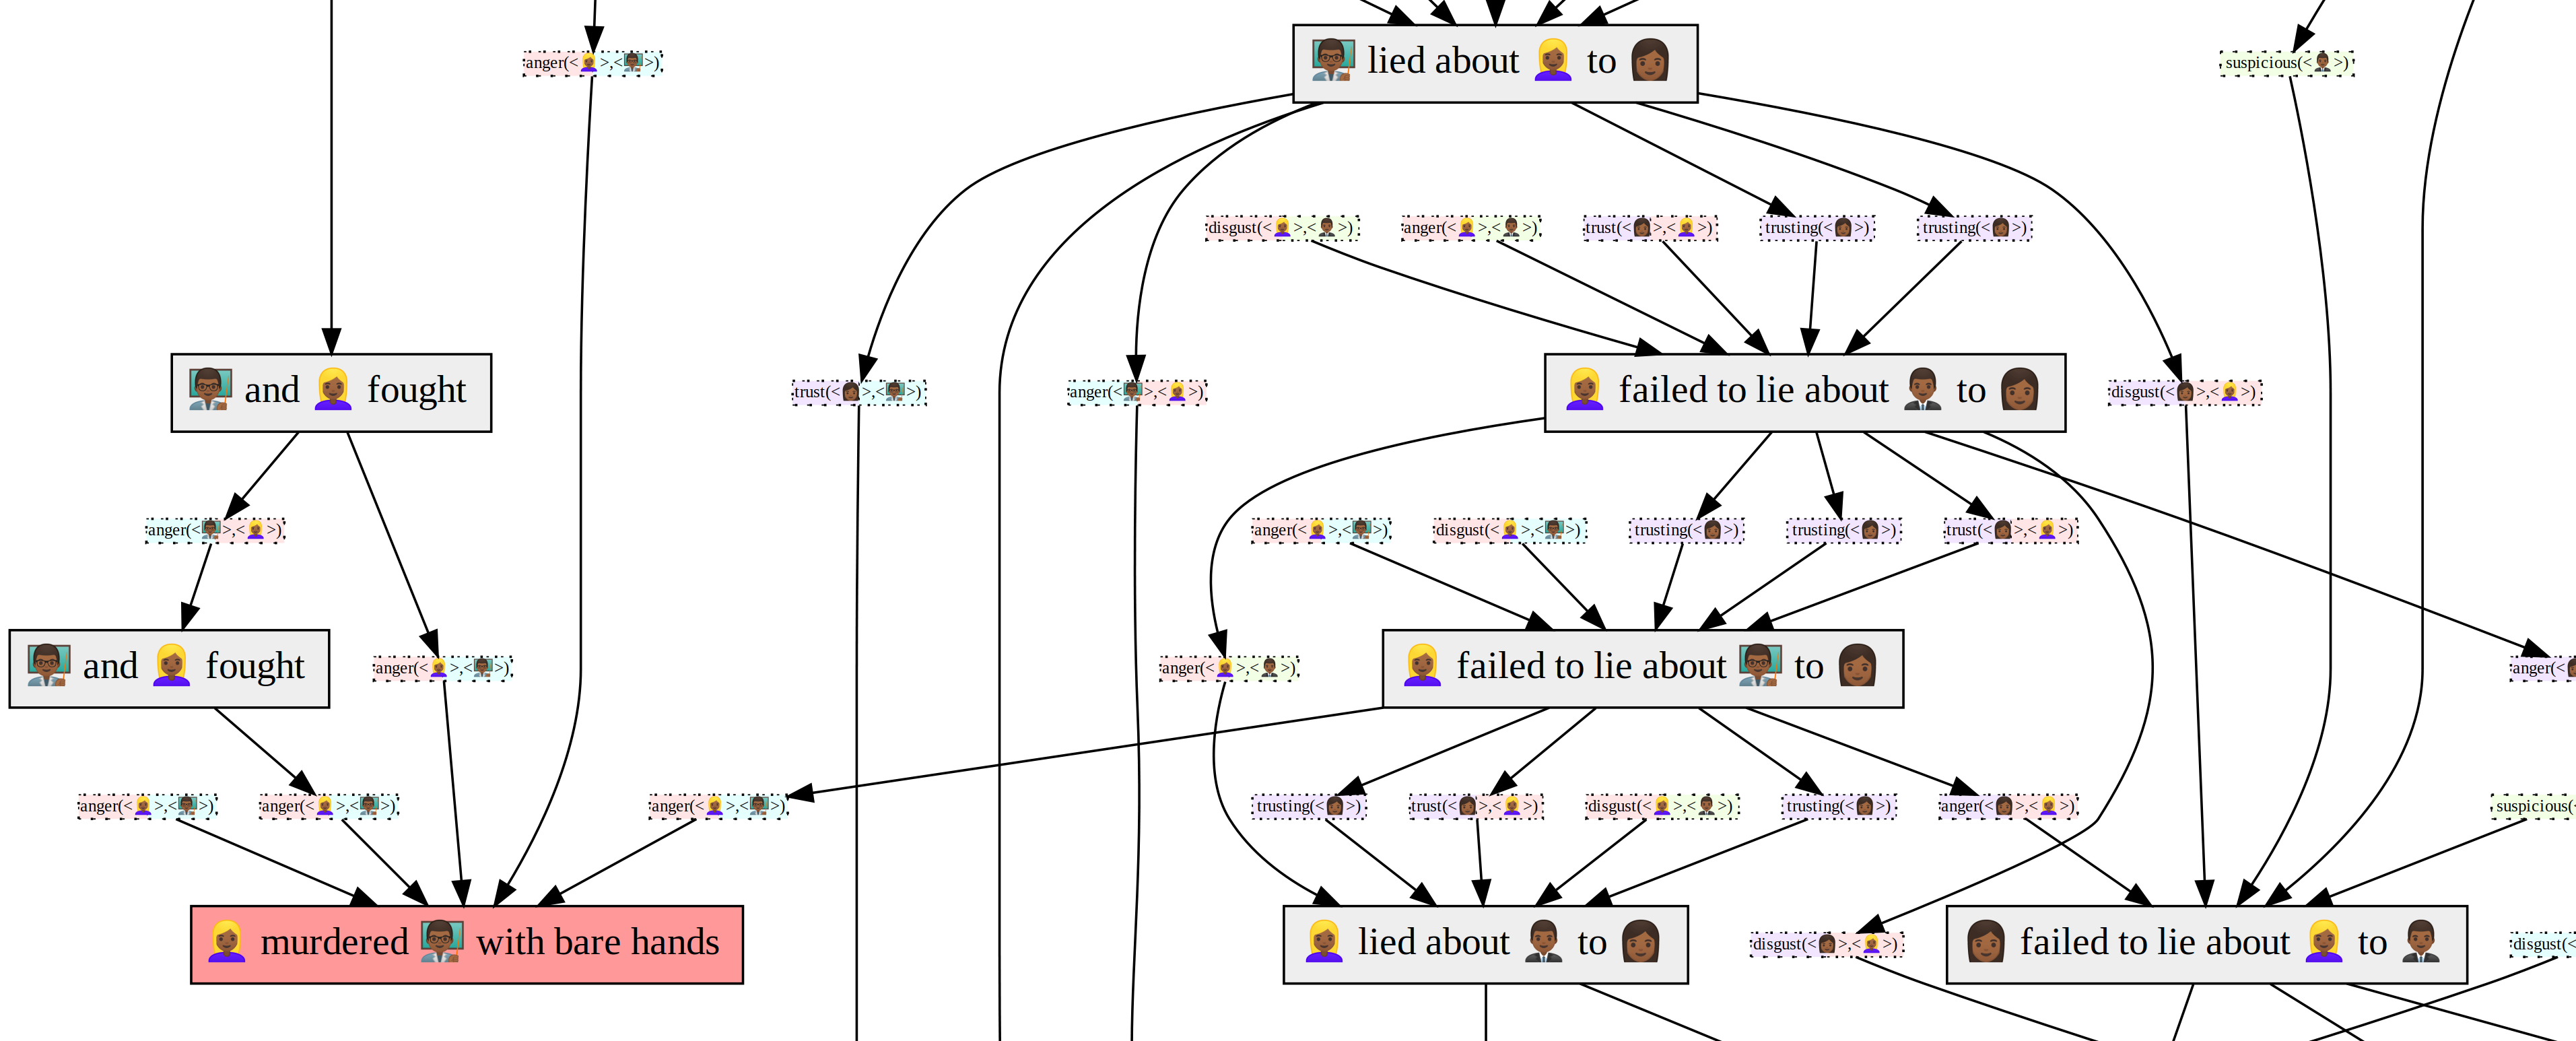
\includegraphics[width=\textwidth]{graph.png}
  \caption{An excerpt from a generated causality graph. The small nodes reflect resources that were generated or existed in the initial state. The larger boxes reflect the actions that agents chose to take. Marked in red is the rule that ended the simulation, the murder.}
\end{figure*}

Our rule authoring system is conceptually identical to that used in Ceptre. We, however, directly compose Python objects, which has the disadvantage of having to adhere to Python's syntax rather than being able to define a domain specific language, but the advantage that we can define functions that group often used sets of predicates, enable domain specific consistency checks, or toggle groups of rules with \enquote{if}-conditions. All of this would have of course also been able to in Ceptre, but would have required introducing new syntactical elements in the Ceptre language, while we effectively work on a meta language level at all times.

Most of the rules pose a dramatic conflict between characters that generate resources like anger or suspicion.
Typically, there is a countering rule that resolves some of this conflict by removing these resources again.
The system is, however, biased towards escalating the conflict quickly, to ensure that stories do not get out of hand and become too complex to understand for a player.
All rules require a motivation as the player would otherwise not have means to follow the flow of events.
For example, fighting with another character requires the preexistence of \enquote{anger} between the two.
Making up would require characters to have developed two \enquote{anger} between each other beforehand, while there also exists a resource of \enquote{trust} between the two.
Further, almost all rules have global preconditions, such as characters being alive or dead or not currently being married when proposing to another character.
These preconditions are modeled in the same way that any other resources are, we did, however, observe that we started thinking about these differently and created macros to help us keep track of this kind of state.\todo{corinna: check new precondition part}

In our current rule set, there are three different motives for murder.
Characters that have many \enquote{anger} resources to another character may choose to murder them over that.
Spouses of characters that are cheating may choose to murder their spouse's lover.
Greedy characters may choose to murder a rich character to acquire their money.
All of these rules require the actor to first acquire a weapon, which delays the inevitable at least for one turn, typically making reason and consequence less obvious in the narrative.
Further, we added one rule where characters may be able to kill another character without being in possession of a weapon if they have particularly many \enquote{anger} resources to another character, to make the \enquote{has\_weapon} predicate slightly less of a definitive indicator of a murder.

Other rules to add substance to the narrative include characters attempting to gamble, which may yield debt that motivates them to acquire money.
This can either be done by attempting to steal from other characters, or even by murdering them.
Characters can seduce each other, become lovers or married, or get divorced.
Further, to make the origin of \enquote{anger} resources that play a central role in the murder motives less obvious, we added the concept of spreading the abstract concept of a lie about another character.
In this way, a character X that does not like another character Y can attempt to spread a lie about Y to a character Z.
If the successful outcome is chosen, Z now also becomes angry at Y.
A more sophisticated system may allow characters to construct specific lies, which would add another layer of interest to the game, as characters would then be able to formulate testimonies which they believe to be true based on information they received from another character, but which the player can then identify as lies.

We added non determinism wherever possible, and in particular to those rules with high rewards for a positive outcome, to ensure that he artificial intelligence will choose options that may have a high pay off for it, but may also result in dramatic tension, as for example, one character catches another in an attempt to steal from them.

Having only few motives for murder does in fact align with the most common structure of Agatha Christie's novels, which we took as a major influence.
Typically, the reason for murder is one of those we listed above, with the depth of the story coming from the elaborate reasoning and the relationships between the characters.\todo{corinna: ref murder reasons in christie novels?}
Putting a focus on delaying the murder for multiple steps is thus important to let agents interact and provide variability to the otherwise few motives.

\subsection{Believable Agents}
In the first iteration of the prototype, we used agents that took actions randomly. This resulted in stories that were varied, but were hard to follow, as no higher level intention of the agents became apparent in the story, only by chance.

To improve the believability of the flow of actions, we added certain rewards to each action that an agent can take. Some actions may incur a penalty, like picking up a weapon which decreases the agent's sanity score, but ultimately may allow it to commit a murder for a reward in fulfillment, if the agent has a fitting motive. The agent's actions became a lot more coherent in this way, as they follow the directions as given by the authored reward structures. With an ability to plan ahead for multiple steps, different agents may try to anger characters about others or find different ways to fulfill the preconditions of the rules with the highest rewards. 

To enable this sort of planned behavior, we used Monte Carlo Tree Search (MCTS) with upper confidence bounds policy (UCB1) \cite{Auer2002}.
We pass the simulation to a MCTS agent, which then expands child states via the upper confidence bounds policy (UCB1)  \todo{tom: piece together}.
Since the simulation has no clear terminal state, we let the simulation play out a fixed number of steps every time instead.
Considering a murder a terminal would have been an option, but this might actually discourage murders from happening, as actors who do not commit a murder get to collect rewards from more steps during playout.
An alternative to this model would have been to only determine win/lose per playout, ending a playout with \enquote{win} if the character commits a murder and \enquote{lose} if they fall victim to one.
This, however, would discourage actors from considering other possibilities that would bring smaller rewards and always steer them towards murder directly.
As such the murder mysteries would get a lot shorter and possibly less interesting if we were to use this strategy.

From experimentation, good values for the maximum number of expanded states is around 100, while the number of playout steps if limited to 10.
Most of the time, simulations will be shorter than 30 steps, making 10 a good balance between performance and allowing actors a good amount of foresight.
The accuracy of the MCTS agents is diminished by the non deterministic choices.
While expanding states, the actor will only get to know a single of those states and assume that this is the outcome.
This is because we store the entire state after each expansion, since the computation of valid moves is costly, so subsequent visits in selection of that node will not make a difference.
In this way, agents will sometimes act more pessimistic or optimistic, based on their once observed outcome of a rule.
As such, we found that not taking another step of optimization to enable the actors to explore all possible outcomes of actions they take, results in a more believable behavior.

With the MCTS agents, we hit significant performance problems as we now had to evaluate valid actions at the current state 300 times more often, with 30 expansions and 10 playout steps. Using pre-calculated hashes for all lookups into the resource state allowed the simulation to progress reasonably fast, at about a pace that allowed a human to follow the event flow as decisions are made. Evaluating decisions via MCTS is typically a fast option \cite{mcts_survey}. This is, however, based on the assumption that calculating rewards is the expensive action, while the random playout is negligible in terms of performance. For our simulation, however, each step of the simulation is costly, as the most expensive action is to find all valid rules, which has to happen on every step of the playout.

On our way to the MCTS agents, we first built an agent system based on OpenAI's \emph{DQN} Q-learning algorithm \cite{baselines}. We set up the state space to reflect all available actions flattened as a two-dimensional array of integers, where each row's first integer corresponds to the constant index of a rule and each column then corresponds to the constant index of a character. A zero in either meant that this rule was unset or this rule did not involve all three characters. The action space then provided the agent with a choice of any of these rules by picking its integer index in the state space array. The challenge that we encountered with this setup primarily comes from the high variability in quantity of the available rules. We put a high negative reward on picking an invalid choice, but, even with a high factor of exploration, only made the agent learn to favor picking the first couple of options that it learned were typically safe. In an attempt to improve this situation, we shuffled the array's rows, such that invalid rules could be found at any index. Here, training over more than three hours did not lead to the agent reliably picking valid rules, which led us to the assumption that the state space was too large to figure out on an automatic basis. More specifically, we offered the agent a state space of 20 rows, with 4 columns each to host the rule index and up to three involved actors. The actor index ranged from 0 to 4 to mark the invalid actor and the 4 valid actor indices and the range of the rule index depended on how many rules the author supplies to the system, which in our case was around 20.

To mention one more attempt we explored, with the motivation of creating a semi-automatic authoring system for rules, we aimed to create a form of completion dialog as found in modern integrated development environments.
To do so, we employed word2vec as a source for word relationships \cite{Mikolov2013EfficientEO}.
Indeed, when tasked with solving word vectors for \enquote{gun} minus \enquote{kill} plus \enquote{cook}, the word2vec system yielded words such as \enquote{wok} or \enquote{dishwasher}.
For this, we used the pre-trained Google News vectors\footnote{https://code.google.com/archive/p/word2vec/}.
In an attempt to have word pairs closer to our domain, we trained our own model with murder mystery stories in the public domain, in our case various Sherlock Holmes stories by Sir Arthur Conan Doyle, as well as early stories by Agatha Christie. Here, we appeared to not have enough data to reach high quality word embeddings: the similarity lookups we tried did not yield usable results.

\subsection{User Interface} \label{user_interface}

We used the Python library Kivy\footnote{https://kivy.org} to develop our user interface (UI).
This allowed us to directly use the Python objects that were created during the murder mystery generation, without the need for serialization when crossing language boundaries.
One important goal during the UI development was to have a very visual representation of the state that is easy to understand for players.
To achieve this, we relied on images to display our characters, objects and rules.
In the beginning we relied on a very small set of sample images for our actors, which quickly led to confusion as the same portrait was used for multiple characters.
Instead we started using emojis as our portraits and other images.
This allowed us to have a great range of portraits that represent different genders, skin colours, ages and occupations.
When assigning the images to the characters, we still proceed mostly randomly, only differentiating between male and female characters.
However, with more than 350 possible images to choose from it is very rare that two characters will look the same.

\begin{figure}
  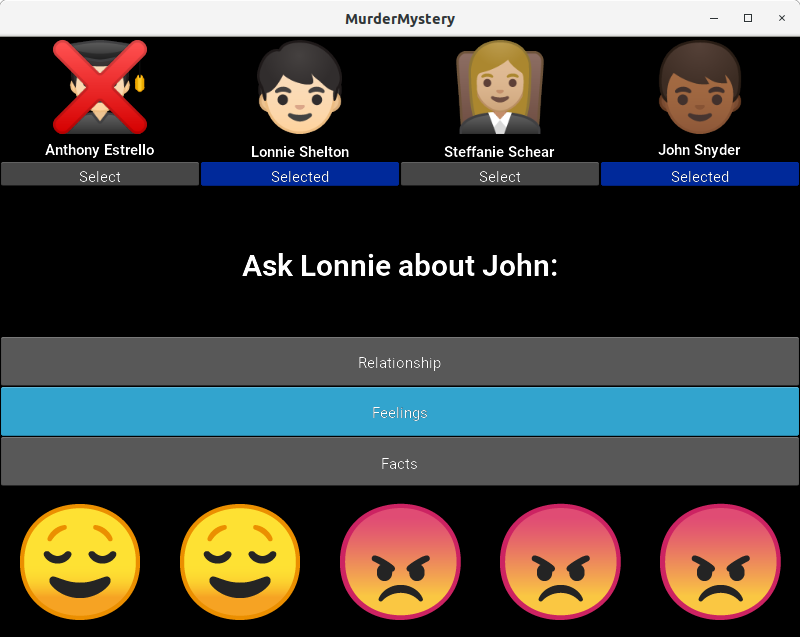
\includegraphics[width=\columnwidth]{feelings_screensot.png}
  \caption{Our user interface. Up top the four involved actors can be seen, with the murder victim crossed off in red. Players may now select characters and choose to ask them questions. In this case the player is asking Lonnie about his feelings towards John. While Lonnie is quite angry with John, there is also a certain level of trust. It is important to note, that the feelings are not necessarily a symmetric relationship.}
  \label{fig:feelings}
\end{figure}

Emojis also allowed us to have uniformity in our other symbols.
Apart from the characters we also use the emojis to represent the emotions and state of relationship between characters.
This has worked very well, as emojis were created to convey these emotions and are well known by the majority of people.
This also allows us to communicate the emotions directly without having to use a level of indirection in the form of text.
Especially if a user plays the game repeatedly, it might quickly become boring if always the same text is being used to explain a specific emotion.
Emojis let us avoid this problem, without having to put a lot of effort into writing multiple versions of one statement.
They also help people to quickly recognize the actors in each action, even if they do not know the names.

\begin{figure}
  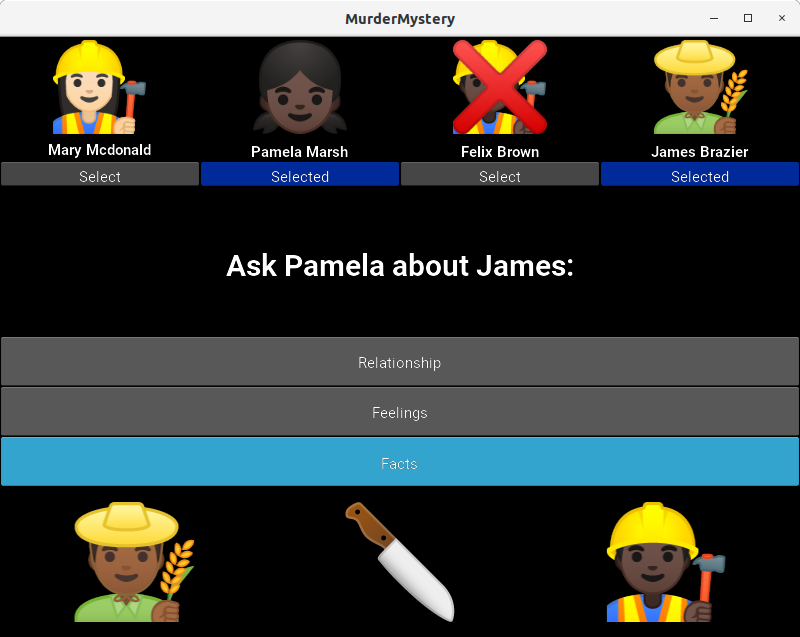
\includegraphics[width=\columnwidth]{murder_screenshot.png}
  \caption{The player is questioning one of the actors, Pamela, on information she has about another actor, James. In this case Pamela knows that James was involved as an actor in the rule \enquote{murder} with another character, Felix, as the victim.}
  \label{fig:murder}
\end{figure}

In addition emojis are used to represent the objects, and the rules which use them.
The rules were harder to represent using emojis.
Some were quite simple, for example murder which we represent simply using a weapon and the two characters involved in the murder, as seen in Figure \ref{fig:murder}.
Others were a bit more complicated, such as the rule \enquote{lie to A about B} which is displayed as the \enquote{secret} emoji.
Unfortunately we were not able to find a recognizable emoji for all rules, for example paying a debt to someone or stealing from someone, which are both represented using different money symbols as they are no other, more obvious ones to choose from.
